\documentclass[a4paper]{report}
\usepackage[landscape, margin=0.5in]{geometry} % marginer og landskap
% Bruk XeLaTex!
%%%%%%% %\XeTeXinputencoding{utf8} % for å få norske bokstaver til å virke
%\usepackage{polyglossia} % språk-pakke
%\setmainlanguage{norsk} % norsk set-up fra språk-pakken

%\usepackage{MyriadPro}

%%%%%% \usepackage{fontspec, xltxtra, xunicode} % pakker for å kunne bruke gitt font
%\setmainfont[Mapping=tex-text]{Myriad Pro}
%%%%%%%%% %\setmainfont{Myriad Pro} % font
%\defaultfontfeatures{Mapping=tex-text}
%\setromanfont[Mapping=tex-text]{Myriad Pro}
%\setsansfont[Scale=MatchLowercase,Mapping=tex-text]{Gill Sans}
%\setmonofont[Scale=MatchLowercase]{Andale Mono}
%\setsansfont{Myriad Pro}

\usepackage[usenames,dvipsnames,svgnames,table]{xcolor} % for å kunne skrive farges slik som i teksten under
\definecolor{ansag}{RGB}{188, 202, 214}  % definerer ANSA-fargene:
\definecolor{ansab}{RGB}{0, 55, 152}
\definecolor{ansar}{RGB}{125, 12, 0}

\usepackage{url} % www-linker
\usepackage[colorlinks]{hyperref} % farger etc. på linker
\hypersetup{colorlinks=true, urlcolor=ansar}
\sloppy % for å bryte opp lange url-adresser

\usepackage{epstopdf} % for å kunne importere .eps filer (grafikk)
\usepackage[gen]{eurosym} % for å få euro-symbol
\usepackage{graphicx}
\graphicspath{./gfx/} % hvor bildene ligger
\usepackage[labelformat=empty, font={it}]{caption} % tar vekk figure_x under bildene + itallic under bildene

\usepackage{flowfram} % selve pakken som lager rammeverket
\vtwotonebottom{0.4cm}{0.3\paperwidth}{[RGB]{125, 12, 0}}{bottomleft}%
{0.6\paperwidth}{[RGB]{255, 255, 255}}{bottomright} %rød linje nede venstre
\htwotoneright{0.8cm}{0.5\textheight}{[RGB]{188, 202, 214}}{sidelright}%
{1\textheight}{[RGB]{188, 202, 214}}{sidenoneright} % grå linje høyre
%\showtypeblocktrue % for å se rammeverket
%\showmarginstrue 
%\showframebboxtrue

\usepackage{parskip} % får ikke tab (indent) på ny linje
\renewcommand{\chaptername}{} % tar vekk kapittelnavn
\renewcommand{\thechapter}{} % tar vekk kapittel nr.
\renewcommand{\thesection}{}
\renewcommand{\thesubsection}{}

\renewcommand{\contentsname}{Innhold}

%\adjustheight{\textheight}
\pagestyle{empty} % tar vekk sidetall i midten på alle sider 
\renewcommand{\chapterfirstpagestyle}{empty} % tar vekk sidetall i midten på første side
\setlength{\columnsep}{1cm} % avstand mellom kolonnene

\usepackage{etoolbox} % slik at neste kapittel kommer på samme side
\makeatletter
\patchcmd{\chapter}{\if@openright\cleardoublepage\else\clearpage\fi}{}{}{}
\makeatother
\makeatletter
%\patchcmd{\@makechapterhead}{\vspace*{50\p@}}{}{}{} % avstand før og etter kapitteltittel
\patchcmd{\@makechapterhead}{\vskip 40\p@}{\vskip 20\p@}{}{}
\makeatother

\NcolumnStop[1]{3}{0.2\textheight}
\Ncolumn[>1]{3}

\setstaticframe{\value{maxstatic}}{label=header, valign=t} % rammebetingelser for overskrift
\newdynamicframe{\textwidth}{\headheight}{0pt}{-\footskip}[footer] % frame for sidetall nederst
\setdynamiccontents*{footer}{\hfill side \thepage\ av \pageref*{lastpage}} % sidetall nederst




\title{Lærestedsbeskrivelse - München}
\author{Henrik Nyhus}
\date{Juli 2013}

\begin{document}

\begin{staticcontents*}{header}
\Huge{\MakeUppercase{\textbf{Lærestedsbeskrivelse}}} 
\hfill 
\includegraphics[scale=1.5]{./gfx/lligg.eps}
\end{staticcontents*}

\chapter{München}

München er hovedstaden i delstaten Bayern, og har gode 1,3 millioner innbyggere. Hvis en regner med forsteder og grensende landsbyer var det per 2007 2,6 millioner innbyggere. Byen er meget velstående, og har mye industri (elektro, bilindustri, kjemi, media/informatikk og øl). Det er en trygg by å bo i, med lite kriminalitet. 

Byen har noe å by på til enhver sesong. Et flertall av parker, 53 museer (blant annet verdens største tekniske museum: Deutsches Museum), 71 teater, mangfoldige årlige kulturarrangementer og flere konsertscener med et utrolig tilbud. En får ikke glemme de to fotballagene FC Bayern og 1860 München. München er ingen typisk storby, og blir av mange kalt Europas største landsby. Den Engelske Hagen er den største parken, og strekker seg mangfoldige kilometer fra byens sentrum nordover. Her sitter det folk og koser seg med piknik og øl, mens andre spiller fotball eller jogger. Sommersesongen avsluttes med Oktoberfest; verdens største øl-festival.
München ligger ca 580 moh, og de nærliggende alpene når man med en times biltur (Tyske alpene; Zugspitze, Lenggries, Spitzingsee). Kjører man en time til er man i Østerrike, hvor man har et ufattelig utvalg av områder til rådighet. Om sommeren er dette fantastiske turområder, og om vinteren fantastiske skiområder.


Byen ligger også meget sentralt til i forhold til Tsjekkia, Sveits, Italia, Ungarn og Østerrike. 

Elven Isar renner gjennom München og langs elven møtes venner og bekjennte for mat, drikke og sportslige aktiviteter. Langs elvebredden finner man fotballbaner og andre sportsrelaterte baner. Man kan svømme i elven, men kun ved oppmerket omeråde. Vannstrømmen er sterk og det skjer årlige drukkningsulykker. 


\begin{figure}[h]
\center
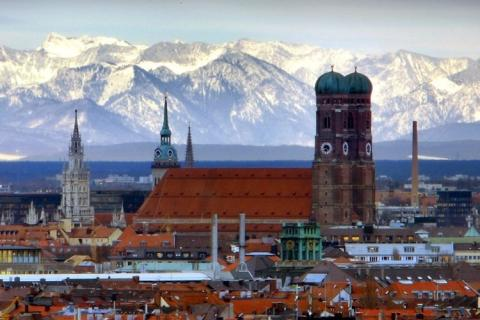
\includegraphics[width=0.31\textwidth]{./gfx/pan}
\caption{Frauenkirche med alpene i bakgrunnen}
\end{figure}




\section{Det tyske folket}
Generelt er tyskere hyggelige og imøtekommende, som nordmann er heller ikke den kulturelle forskjellen så stor. Tyskere er svært opptatt av orden og byråkrati, noe som til tider kan virke overdrevent. Den tyske humoren er noe annet hva man ser i Norge og det kan ta litt tid før man får dreisen på tankesettet. 

I de sørlige delstatene, Bayer og Baden-Württemberg, er man mer konservativ i forhold til de andre tyske delstatene. Titler og høflighet ( Sie- og du-form) er mer utbredt her, dette gjelder spesielt ovenfor proffesorer, politi og andre autoriteter.
Fyll og fest er på et roligere og et mer ''anstedig nivå'' og tyske jenter drikker langt mindre enn norske jenter. Hvordan man går kledd vil også bli, i langt større grad enn i Norge bedømmt. Det er uvanlig å se studenter i joggebukse eller tights. 
Alt dette kan virke som småpirk og noe man ikke trenger å ta hensyn til, men det blir lagt merke til. 



\section{Språket}
Tysk er generelt for nordmenn ikke spesielt vanskelig, tyskere bryr seg heller ikke så mye om man sier noe gramatisk feil så lenge det er forstålig. I starten kan det være uvant å prate tysk, men som tiden går blir man fort flinkere og alt løsner opp. Nordmenn har som regel lite problem med den tyske uttalelsen og tyskere selv skjønner ikke at de snakker med en utlending. Noen tilfeller kan det være lurt å fortelle vedkommende at man ikke er tysk, og ikke en beruset person.

Nesten alle studier i München foreleses på tysk.
Man må fremlegge dokumentasjon på at man kan nok tysk for å bli immatrikulert.
Det betyr at man må ha et DSH prøve med resultat 2 eller bedre, TestDaF med 4.4 eller bedre, Goethe med ZOP eller et diplom fra lignede institusjoner. 

En liste over noen språkkurs som godkjennes i München finner du her:\\
\url{http://www.uni-muenchen.de/studium/studium_int/studium_lmu/sprachkurse/andere_empf_deutsch/}


Her er en liste over noen godkjente språkprøver:\\
\url{http://www.uni-muenchen.de/studium/studium_int/studium_lmu/bewerbung/20_dt_nachw/}

En får tilbud om å ta en prøve rett før studiet begynner/rett før søknadsfristen. Dette kan man også ordne selv i forkant, enten i München, eller f.eks. ved Goethe-Institut i Oslo.
En skal ikke undervurdere den språkkunnskapen som trenge for enten å bestå en språkprøve eller å faktisk studere på tysk. Akademisk tysk er ikke som tysk C-språk!
  Det er ikke uvanlig å komme ned ett semester før en tenker å begynne å studere for å forberede seg og bli kjent med byen.

Dokumentasjon på påkrevd tyskkunnskap skal ved immatrikulasjonen vises. Det er helt greit å søke uten å ha beviset.

Lånekassen gir støtte til et forberedende språkkurs! \\
\url{http://www.lanekassen.no/Hovedmeny/Stipend-og-lan/Utland/Hvor-mye/Sprakstipend/}

\begin{figure}[h]
\center

\includegraphics[width=0.15\textwidth]{./gfx/wappen}
\caption{Byvåpenet til München}
\end{figure}

\subsection{Dialekt}
Bayersk kommer i flere former og varierer i forhold til hvor personen er oppvokst. Lokalbefolkningen i München by snakker mer høytysk og er lette å forstå, derimot kan man treffe på proffesorer eller klassekamerater, som snakker bredt og nekter å endre på det. Flere tyskere som bor i Norge mener bayersk samsvarer med trøndsk. 
Men det går som regel veldig bra og er ikke et stort hinder.




\section{Ulemper ved å bo i utlandet}

Reise fra venner og familie til et sted hvor man har lite/ingen bekjennte. Feriene i Tyskland er helt anderledes enn i Norge, bortsett fra juleferien. Man har semesterferie fra tidlig feb. til sent april og sommerferie fra tidlig august til sent oktober. Dette gjør samkjøring av ferieplaner med norske venner/familie utfordrende. Det er nok enklere å studere på morsmålet, men det betyr ikke at det heller er vanskelig å studere på tysk. Det er mange som gjør det, og ende flere som har gjort det før deg. Det er veldig kult å kunne prate flytende tysk.

Ellers: Smil til livet, og livet smiler til deg.

% !TeX spellcheck = de_DE
\chapter{ANSA}
Når mamma og pappa er 5400 km unna...
Alle som studerer utenlands vil støte på store eller små problemer underveis. Noen problemer løses lett ved en telefon hjem til mor og far. Husk at også vi er her for deg mens du er ute i verden og studerer. \\
\url{http://www.ansa.no}


\section{Hva kan ANSA hjelpe deg med?}
Du kan bli medlem av ANSA når du har fått en studieplass i utlandet. Som medlem kan du tegne ANSA Studentforsikring og ANSA Pluss og du kan delta på våre arrangementer i Norge og utlandet. Du får også rådgivning hvis du får problemer under studieoppholdet, tilsendt medlemsbladet ANSAnytt i posten og jobbtilbud på e-post.
Trenger du bistand i forhold til problemer i studielandet eller informasjon om forhold og instanser i Norge, kan du ta kontakt med ANSAs rådgivere. Kontakt rådgiverne per e-post eller per telefon 22 47 76 00.


\begin{figure}[h]
\center

\includegraphics[width=0.31\textwidth]{./gfx/isar}
\caption{Tørste sjørøvere på tokt i Isar}
\end{figure}





\section{ANSA München}
Vi er omlag 12 heltidsstudenter og langt flere utvekslingsstudenter. De fleste har god kontakt med hverandre. De fleste studerer medisin, i tillegg er det noen som studerer informatikk, matematikk eller andre ingeniørfag.

Hvert år arrangerer vi 16. mai - russefest, juletrefest og felles turer. Det Norske Konsulatet står for 17. mai, og svenskene treffer vi på St. Hans.
ANSA arrangerer semester-kickoff hver semesterstart, og treffes jevnlig i semesteret. Det er et par sentrale norske personer (ikke bare ANSA-medlemmer) som organiserer disse jevnlige "Stammtischene". Informasjon om dette finner en i vår facebookgruppe "Norwegischer Stammtisch München / ANSA München". Her opplyses det altså om de vanlige "Stammtischene" og ANSA-arrangerte events. Her blir alle som vil komme; venner, kjente og norsk-interesserte invitert. Hvis det er noe som er kun ment for ANSA-medlemmer, går dette over e-mail.\\
\url{http://www.ansa.no/ANSAland/Tyskland/Lokallag/ANSA-Munchen/}

Facebook:\\
\url{http://www.facebook.com/groups/2244635897}

\section{Russefest}

bla bla

\section{17. Mai}
\begin{figure}[h]
\center

\includegraphics[width=0.31\textwidth]{./gfx/17mai}
\caption{Nordmenn i tog ved Chinesischer Turm i Englischer Garten}
\end{figure}


\section{Juletrefest}


\section{Isar River-run}
bla bla hvert år,.. s-bahn osv.



\section{Norwegerfete}

blablabla




\section{Hva koster medlemskap i ANSA?}

\begin{enumerate}
\item Halvårsmedlemskap (vår/høst) koster 250,-.
\item Skoleårsmedlemskap (dvs. fra 1. juli til og med 31. juli året etter) og kalenderårsmedlemskap (dvs. fra og med 1. januar til og med 31. januar året etter) koster 375,-.
\item Tegner du medlemskap for flere år av gangen er prisen:
\begin{enumerate}
\item 2 år: kr. 645,- 
\item 3 år: kr. 865,-
\item 4 år: kr. 975,-
\item 5 år: kr. 1125,-
\item 6 år. kr. 1275,-
\end{enumerate}
\end{enumerate} 


\section{ANSA Forsikring}
Hva må til for at jeg kan tegne ANSA forsikring?
For å kunne tegne ANSA studentforsikring må du være medlem av ANSA, samt være medlem av norsk folketrygd, eller ha rett til utvidet stønad til helsetjenester NAV internasjonalt.

\subsection{Hva koster forsikringen?}
ANSA studentforsikring er delt inn i en Nordengrunnpakke, Europagrunnpakke og en Verdensgrunnpakke. I tillegg kan man tegne en valgfri sykeforsikring i tillegg til Europa- eller Verdensgrunnpakken. Forsikringen kan tegnes for enten 4, 6 eller 12. måneder. Prisinformasjon finner du på \url{www.ansa.no/forsikring}.

\subsection{Hva dekker forsikringen?}
ANSAs studentforsikring er spesialdesignet for utenlandsstudenter og består blant annet av innbo-, ulykke- og studieavbruddsforsikring, samt forsikring som dekker hjemkallelse og reisegods. I tillegg kan man tegne en valgfri sykeforsikring.

\section{Studentavis}
Norwegern er avisen for norske studenter i Tyskland. Den skal utgis to ganger i året, i begynnelsen av vintersemesteret, vanligvis på organisasjonskurset, og i begynnelsen av sommersemesteret, her blir den utgitt på landsmøtet.
Oppmøtte ved organisasjonskurset og landsmøtet tar med seg aviser og deler ut til medlemmene i sin by, ellers blir avisene sendt ut. Har du ikke fått avisen? Send en email til redaktøren, så blir det en ordning på det!
Avisen skal være selvforsørgende, dvs at utgiftene skal dekkes av reklame i avisen. Har din bedrift lyst til å støtte avisen og reklamere? Ta kontakt med markedsansvarlig her.
På denne siden vil du finne de siste utgavene av Norwegern og artikler fra eldre utgaver. God fornøyelse!

\begin{figure}[h]
\center
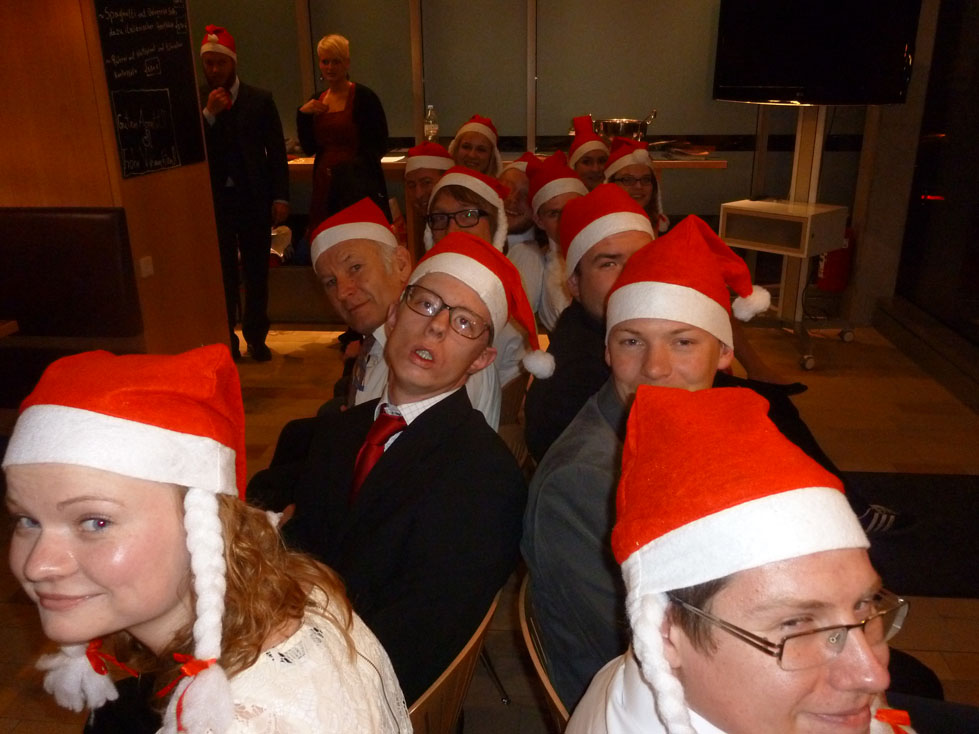
\includegraphics[width=0.31\textwidth]{./gfx/juletrefest}
\caption{Nisser klare for stolleken}
\end{figure}

\section{Sjømannskirken}
Sjømannskirkene og ANSA har utviklet en beredskapsplan for tilfeller der det skjer ulykker i utlandet. Beredskapen består for vår del av presidenten i ANSA, medlemsservice, infosenteret, rådgiverne og studentprestene, som jo hører under Sjømannskirken. Hvis du står ovenfor en ulykke eller en katastrofe av noe slag, gjør du klokt i å ringe enten presidenten eller studentpresten din. Disse vil ringe og kontakte de andre i beredskapsgruppa. De varsler også UD. Det neste de gjør er åsjekke om det finnes studenter hvor ulykken inntraff og kontakter disse. I tillegg diskuteres hva som bør gjøres og de avventer nærmere beskjeder.

\begin{figure}[h]
\center
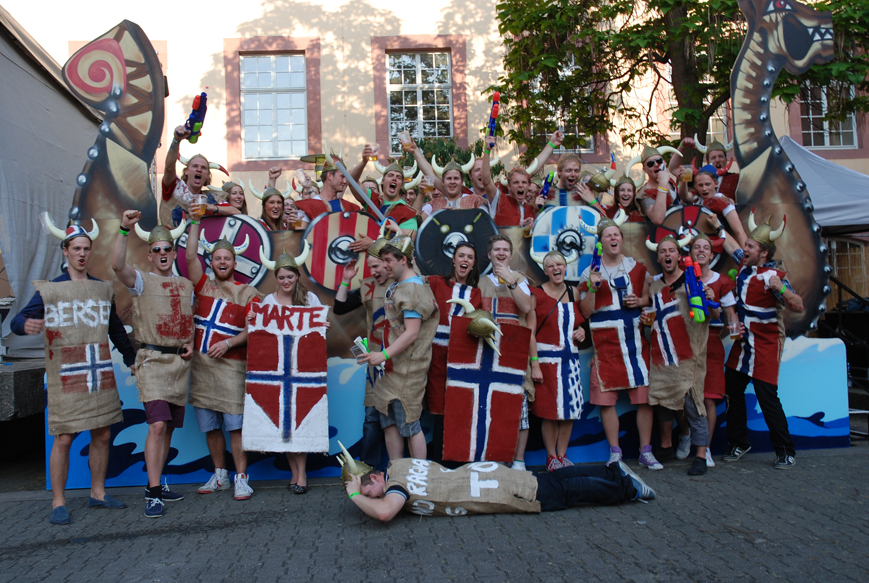
\includegraphics[width=0.31\textwidth]{./gfx/norwegerfete}
\caption{Norwegerfete i Mannheim}
\end{figure}

\chapter{Studere}
Her er en generell brosjyre fra LMU som en bør lese gjennom:
\url{http://www.uni-muenchen.de/studium/studium_int/studium_lmu/immatrikulation/engl10getstart.pdf}


\section{Semesterordning}
Semesterordningen er ganske annerledes enn i Norge; vintersemesteret (WS) begynner ca. 15. oktober og varer til ca. 15. februar, og sommersemesteret (SS) fra ca. 15. april til ca. 15. juli, så semesterferiene er lange og fine. Likevel må noen av disse brukes til eksamen, da alle store eksamener (Staatsexsamen, Physikum, Zwischenprüfung, Vordiplom osv.) blir holdt etter semesterslutt. Medisinstudenter, veterinærstudenter og andre må og bruke noe av denne tida til å gjennomføre obligatoriske praksisperioder.

\begin{figure}[h]
\center
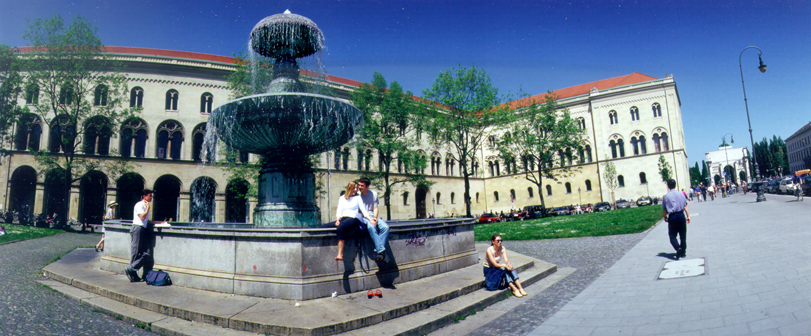
\includegraphics[width=0.31\textwidth]{./gfx/lmu}
\caption{Hovedbyggningen til Ludwig-Maximilians-Universität}
\end{figure}

\section{Utdanningsinsutisjoner}
Det er et stort utvalg av høyskoler i München. De tre største er Ludwig-Maximilians-Universität (LMU), Technische Universität (TUM) og Hochschule München (FHM). LMU og TU er to av Tysklands ni eliteuniversiteter med henholdsvis 45.000 og 25.000 studenter.


LMU - \url{http://www.uni-muenchen.de}\\
TUM - \url{http://portal.mytum.de}\\
FHM - \url{http://www.fh-muenchen.de}\\

Andre:
\begin{enumerate}
\item Hochschule für Politik \\
\url{http://www.hfp.mhn.de}
\item Akademie der Bildenden Künste \\
\url{http://www.adbk.de}
\item Hochschule für Musik und Theater \\
\url{http://website.musikhochschule-muenchen.de/}
\item Bayerische Theaterakademie August Everding \\
\url{http://www.theaterakademie.de}
\item Hochschule für Fernsehen und Film \\
\url{http://www.hff-muenchen.de}
\item Universität der Bundeswehr \\
\url{http://www.unibw.de}
\item Munich Business School \\
\url{http://www.munich-business-school.de}
\end{enumerate}




Informasjon om andre utdanningsinstitusjoner finner man blant annet her:

\url{http://de.wikipedia.org/wiki/M\%C3\%BCnchen#Hochschulen_und_Forschungseinrichtungen/}\\

\url{http://www.muenchen.de/themen/bildung/hochschulen.html}



\subsection{Studietilbud}
Hver høyskole har sitt eget utdanningstilbud som er tilgjengelig på deres respektive internettsider. Her finner man så å si alt en kan tenke seg. 
I 2006 startet begynte høyskolene i München å gå over ifra det gamle Diplom- studiet til Bachelor og Master som vi kjenner i fra Norge.
NB! Enkelte fag kan bare starte til vintersemesteret (bl.a. medisin).



LMU\\
 \url{http://www.uni-muenchen.de/studium/studienangebot/}\\

TUM\\
 \url{http://portal.mytum.de/studium/studiengaenge/index/}\\

FHM \\
\url{http://www.hm.edu/studieninteressiert/studienangebote_1/bersicht_10/}




\section{Søknadsprosessen (ved LMU)}
Det er fire inndelinger for studier ved LMU (for de andre høyskolene i München; sjekk deres internettsider)

1 - Frie studier: søknad til høyskolen (papirformat, karakterer teller ikke)
Her er informasjon og søknadsskjema (link til en annen side): \\
\url{http://www.uni-muenchen.de/studium/studium_int/studium_lmu/bewerbung/}

Søknaden sendes til det Internasjonale Kontoret ved LMU.

Liste over frie studier: \\
\url{http://www.uni-muenchen.de/studium/beratung/vor/studienplatz/studienplatz/zulassungsfrei/}





2 - Lokalt opptaksbegrensede studier må man må søke til høyskolen (karakterer teller)

Man søker kun online, altså ikke papirformat. Her søker man:\\
\url{http://www.uni-muenchen.de/studium/hochschulzugang/bewerb_einschreib/verfahren/online_bewerb/}


3 - Sentralt opptaksbegrensede studier må man er søker til et landsdekkende sentralt opptak, ikke til den lokale høyskolen (lignende samordna opptak - karakterer teller)

Her søker man: \url{http://www.hochschulstart.de}

Informasjon fra LMU om begrensede studier: \\
\url{http://www.uni-muenchen.de/studium/hochschulzugang/bewerb_einschreib/zulassungsbeschr/bundesweit/eu/}

Liste over studier som er begrenset:
\url{http://www.uni-muenchen.de/studium/beratung/vor/studienplatz/studienplatz/zulassungsbeschr/index.html}


4 - For studier med spesielle opptaksprøver ("Studiengang mit Eignungsprüfung"), se studiegang for mer informasjon.



\section{Frister}
Sommersemester:  15. juli
Vintersemester: 15. januar

\begin{figure}[h]
\center
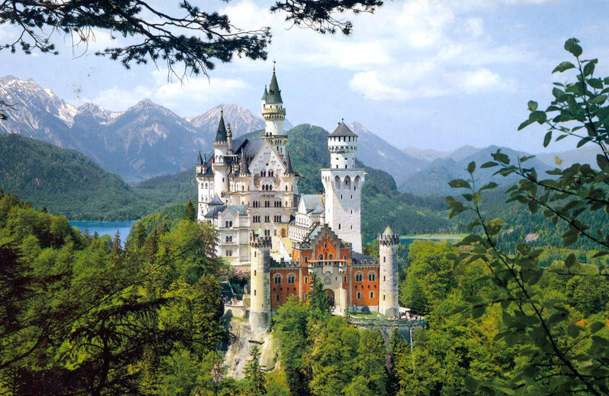
\includegraphics[width=0.31\textwidth]{./gfx/neu}
\caption{Scloß Neuschwanstein ligger ikke langt i fra München}
\end{figure}


\section{Immatrikulasjon (ved LMU)}
De som har søkt og fått plass, trenger bare møte opp til gitt termin med de nødvendige papirene for å skrive seg inn. 
Det er en del papirer en skal ha med seg. Ikke minst diplom på bestått språkprøve. Alt dette foregår i hovedbygningen til LMU.

Nødvendige papirer:
\begin{itemize}
\item Opptaksbrev
\item Online-formular (se nede)
\item Pass
\item Vitnemål (generell studiekompetanse, oversatt til tysk med rett kopi)
\item Sykeforsikringsbevis (se nede, ta med Europeisk helsetrygdkort)
\end{itemize}



Sykeforsikringsbevis får man ved å ta med seg EU Helsekortet sitt til en "krankenkasse" (fritt hvilken) hvor en får et papir som sier "Denne personen er forsikret". De er normalt i samme lokalet og vil være tilgjengelig til samme tid man kan skrive seg inn. Dette er en ren formalitet, koster ingenting og man må ikke nødvendigvis bruke den "Krankenkassen" hvis noe skulle skje. 
Europeisk helsetrygdkort får man fra NAV, men det kan ta opptil to uker fra man søker til man får det i posten. Kortet er gyldig i flere år.

En oversikt over de vanligste Krankenkassene:\\
\url{http://www.uni-muenchen.de/studium/studium_int/studium_lmu/bewerbung/40_eu_auslaender/}

Informasjon om immatrikulasjonen (nødvendige papirer etc.) finner du her:\\
\url{http://www.uni-muenchen.de/studium/studium_int/studium_lmu/immatrikulation/}


Nødvendige dokumenter:\\
\url{http://www.uni-muenchen.de/studium/studium_int/studium_lmu/immatrikulation/grundl_unterlagen/}

Før en går for å immatrikulere seg, må alle ha fylt ut dette online:\\
\url{http://www.uni-muenchen.de/studium/hochschulzugang/bewerb_einschreib/verfahren/online_einschreib/online_einschreibung/}

Som utlendning møter man først opp ved det internasjonale kontoret, for å få vitnemål kontrollert. Deretter går man over til "Studentenkanzlei", som er i nabobygget (sammen med Tyskerne). Informasjon om hvor og når får man i opptaksbrevet.

Avdeling for internasjonale studenter:\\
\url{http://www.uni-muenchen.de/studium/kontakt/international/}

Dette er som sagt hvordan det gjøres ved LMU. Informasjon om hvordan søknadsprosessen og immatrikulasjonen ved andre høyskoler i München foregår finnes på deres respektive internettsider.


\section{Medisinstudiet}

Det er opptak kun en gang i året, om sommeren. Det er omtrent 1000 studenter som begynner på medisin hvert år. Studiet deles inn i en førklinisk del , og en klinisk del. I den førkliniske delen av studiet, som er normert til 2 år, er de tre store og viktige grunnleggende fagene anatomi, fysiologi og biokjemi. Som regel er ikke forelesningene obligatoriske, men i de fleste fagene er det kurs, som en må stille opp på. Prøver er det også, som regel multiple choice.
I feriene må det til sammen utføres 3 måneder med pleietjeneste på et sykehus. I hvilket land denne praksisen avlegges, er det samme, så lenge det er på et sykehus. Når alle prøvene i fagene er bestått, og praksisen gjennomført, kan man melde seg opp til "1. Staatsexamen" også kalt "Physikum". Den består av en skriftlig del (multiple choice) som går over to dager. I tillegg er det en muntlig del. En blir da eksaminert i de tre store fagene.
Når "Physikum" er bestått, dvs. både den skriftlige og muntlige delen, kommer man til den kliniske delen av studiet. Denne er normert til 4 år. Både LMU og TU tilbyr denne delen av studiet. TU er litt mindre. Den kliniske delen er mye mer praktisk rettet. Ikke minst etter innføringen av den nye approbationsordningen, har studentene mye kontakt med pasienter og blir kjent med sykehuset fra innsiden. I feriene må en i løpet av de tre første årene ha 3 måneders praksis på et sykehus og en måneds praksis hos en fastlege. Det siste året av studiet, er et "Praktisches Jahr". Da jobber man på et sykehus, en tredjedel av tiden må en jobbe i kirurgien, en tredjedel i indre medisin, og den siste tredjedelen kan man velge selv hva man vil jobbe med innenfor medisin. Etter det praktiske året, kommer "2. Staatsexamen" også kalt "Hammer Examen". 

Når en har bestått dette, er man ferdig utdannet lege i Tyskland. Vil en tilbake til Norge rett etter studiet, må en ha vanlig norsk turnustjeneste!

Dersom du er interessert i å studere i München eller du allerede har fått studieplass her, må du ikke nøle med å ta kontakt hvis det er noe du lurer på!


\section{Oversetting og kopiering}

Når du skal søke på skoler i utlandet, vil du som oftest bli bedt om å sende med godkjent kopi av vitnemål oversatt til landets språk. Det er mulig at det behandlende organ ved universitetet også aksepterer vitnemål på engelsk. Du vil finne informajson om dette på søknadssidene til universitetet.

Oversettelsen må i de fleste tilfeller være utført av godkjente oversettere.  Oversetting hos byrå eller translatør kan koste fra kr. 600 til kr. 1000 per ark. Spør derfor først ved din videregående skole om de kan oversette vitnemålet ditt til det språket du ønsker det på. Universiteter og høgskoler kan stort sett gi deg en karakterutskrift på andre språk enn norsk. Enkelte vidregående skoler kan oversette vitnemålet til tysk, spør skolen og hør om de kan gjøre det for deg.
Du kan henvende deg direkte til en statsautorisert translatør for å få oversatt vitnemålet ditt, eller du kan bruke et oversetterbyrå som har statsautoriserte translatører. Prisnivået hos byråer vil ligge noe over prisen du får direkte hos en statsautorisert translatør. 


\subsection{Attester}
Hør først med de som har utstedt attesten om de kan skrive den på et annet språk. På lik linje med vitnemål, kan attester også oversettes av en statsautorisert translatør, evt. hos et byrå som har statsautorisert translatør.

\subsection{Rett kopi}
Det er få offentlige kontorer i Norge som idag er villige til å stemple rett kopi. Det er derfor lurt å høre med skolen du har gått på i Norge om de kan ta kopi av vitnemålet og stemple dette for deg. En kan også få rett kopi hos NAV, politiet, flere biblioteker og enkelte kommunesentere.




\chapter{Økonomi}

\section{Priser og finansiering}
Dagligvarer er mye billigere enn hva man finner i Norge, det er rundt halv pris på det meste. Alkohol og tobakk er mye gunstigere, 
en 0,5 liter øl på byen koster rundt 23-30 kroner.
Priser på leie av leilighet varier i forhold til beliggenhet, størelse og tilstand, men for rundt 4000 kroner får man en sentral leilighet.

\begin{figure}[h]
\center
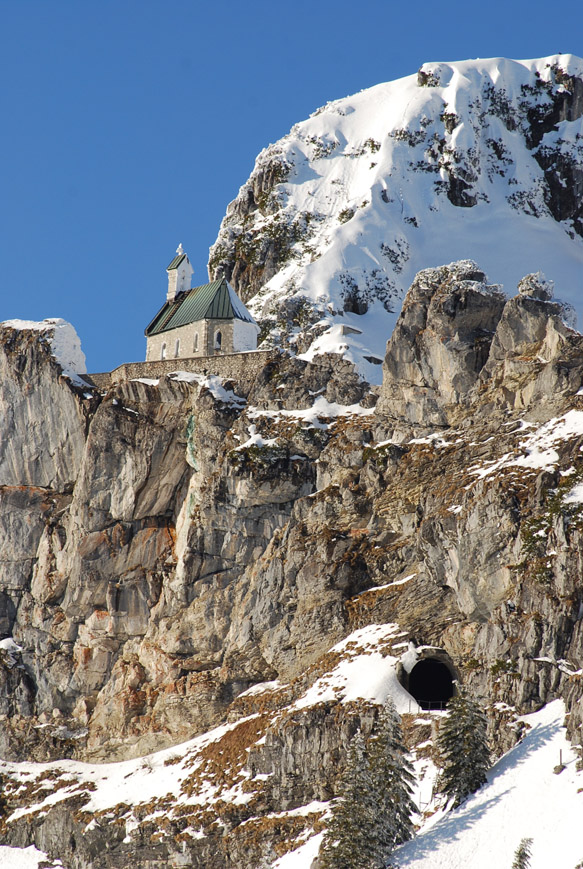
\includegraphics[width=0.2\textwidth]{./gfx/wendelstein}
\caption{Kirken på Wendelstein ligger høyest i Tyskland. Her er det meget god offpist-kjøring om vinteren.}
\end{figure}

\section{Lånekassen}
Du kan få støtte av lånekassen til å studere språk fra tre til fem mnd før studiestart. Dette kalles tilretteleggingssemester. Har du kommet inn på et studie kan du få språkstipend før studiestart .


 Du vil kunne få økonomisk støtte fra Lånekassen så lenge utdanningen din kan:
 
 
\begin{enumerate}
\item Utdanningen må tilsvare, være på nivå med, eller kan bli godkjent som en del av en norsk bachelor- eller mastergrad.
\item Lærestedet må være offisielt godkjent i studielandet.
\item Utdanningen må være på fulltid.
\end{enumerate}
 
 
Utdanningsstøtten er 90 800 kroner årlig og blir gitt som lån. 40 \% av støtten omgjøres til stipend forutsatt at alle eksamener er bestått (54 480 kroner er lån, 36 320 kroner er stipend).
Til høyere utdanning kan du få stipend til to tur-retur reiser, men ikke mer en 7250 kroner per studieår. Egenandelen er 2 080 kroner per studieår. 
Reisestipendet blir automatisk beregnet når du søker om stipend eller lån



\section{Privat stipend}
Se \url{http://www.legathandboken.no}. \\
Forskningsrådet deler hvert år ut stipender til studenter på som vil studere i Tyskland. Se Forskningsrådet for mer informasjon. \\
\url{www.forskningsradet.no}

\begin{figure}[h]
\center

\includegraphics[width=0.2\textwidth]{./gfx/russefest}
\caption{Haugalending på russefest ved Monopterosen i Englischer Garten}
\end{figure}

\section{Skolepenger}

I München betaler man skolepenger, men disse er svært lave og ligger på rundt 500 Euro. I tillegg må du betale en semesteravgift på mellom 50 og 200 Euro. Lånekassen gir utdannings- og skolepengestøtte til bachelor- og mastergrader ved offentlige godkjente læresteder for høyere utdanning i Tyskland. Du kan også få støtte til å ta deler av en norsk utdanning (utveksling) i Tyskland. For å få støtte fra Lånekassen, må du immatrikuleres som regulær student ved det tyske lærestedet.

Det er mulig at kravet om betaling av skolepenger vil frafalle i 2013/2014. Sjekk universitetets hjemmeside for informasjon om dette.



\chapter{Bo}
Her er en liten "ordbok" som kan komme til hjelp:
\begin{itemize}
\item Wohnung/Leilighet/WG (Wohngemenischaft) - Bofellesskap/Kollektiv
\item Kalt Miete/warm Miete - uten og med strøm/varme inkludert i leieprisen
\item Zwischenmiete - noen som er borte for en periode og leier ut leilighet/rom
\end{itemize}

Dersom man skal ned for språkkurs og trenger bolig, har de fleste lærestedene gode løsninger.

\url{http://www.goethe.de/ins/de/ort/mue/unt/}


IKKE betal leie på forhånd, det er nok av tilfeller hvor studenter betaler leie for et semester også viser det seg at de har blitt rundlurt. 
Det er også svært lurt å ha en leiekontrakt og faktisk vite hva man signerer på.


\section{Pris}
Boligmarkedet er presset, og prisene kan være ganske høye. Skal en leie privat må en regne med å betale ca. 450 \euro{} i måneden, men det er selvsagt mulig å finne noe som er billigere. 

\section{Hvor finne leilighet}
Gjennom universitetet og studentsamskipnaden (Studentenwerk) kan en søke om plass på forskjellige studenthjem, med forskjellig standard, pris, plassering og ventetid. Hos Studentenwerk på Giselastraße kan en forhøre seg og få hjelp til dette (se hjemmeside).
På de mest populære må en kanskje venta 1,5 år, men det finnes gg steder hvor ventetiden er mindre enn et semester. En leilighet på 15 m2 med eget bad og kjøkken (10 minutter fra sentrum med U-Bahn) kan koste 250 euro. Noen av studenthjemmene ligger i sentrum, men de fleste er litt utenfor byen. De største studentbyene er Olympiadorf, Studentenstadt og Großühadern. Buss-, U-Bahn-, S-Bahn- og Straßüenbahn(trikk)-nettverket er så godt utbygd at avstandene for de fleste ikke blir noe problem. Alt som du kan nå med U-Bahn er bra, S-Bahn dekker et meget stort område, så de ytre stasjonene kan være et stykke utenfor sentrum.

\url{http://www.studentenwerk-muenchen.de/wohnen/}\\
\url{http://www.studentenwg.de}\\
\url{http://www.wg-gesucht.de}





\section{Når bør jeg begynne å lete?}
Bolig er noe av det som kan være litt kinkig å organisere (i hvert fall ifra Norge). Et godt tips: Vær tidlig ute! Altså ihvertfall en måned før studiestart.


\begin{figure}[h]
\center
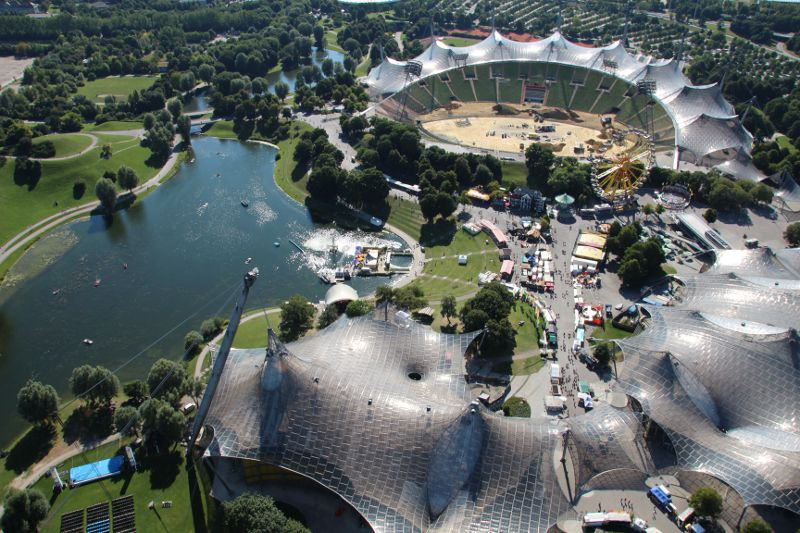
\includegraphics[width=0.30\textwidth]{./gfx/olympia}
\caption{Olympiapark ble bygget til OL i 1972}
\end{figure}


\section{Typer bomuligheter}
Det er helt smak og behag hva som er den beste løsningen for hver enkelt person. Wohngemeinschaft/WG eller kollektiv som det heter på norsk er ofte en mer sosial løsning enn å bo alene. Det kan innebære støy og andre plager, men er billigere og som sagt mer sosialt enn å bo alene. Pris rundt 400 \euro{}

Studentenheim er nok den billigste løsningen og man har som regel en egen, noe mindre, hybel. Her bør man være litt på vakt, det er flere katolske og andre former for studentenheim som har egne regler, angående besøk av kjærester og annet.
Ventelistene er ofte lange og man må vente opptil et til to år før det er en ledig hybel.
Pris rundt 300 \euro{}

Man kan også velge å bo alene, den dyreste og minst sosiale løsningen. Passer kanskje til den som er noe mer reservert, men kan fort bli litt ensomt og lite kontakt med tyskere . På den andre siden er man bedre vernet fra bråk og forstyrelser.
Pris rundt 450 \euro{}

Hva skal man velge? det må du finne ut selv!



\chapter{Transport og reise}

\section{Fly}
SAS og Norwegian flyr fra flere store byer i Tyskland. Bestiller man i god tid, kan man få billetter til og fra München til under tusenlappen.
Hvis man er litt sent ute og flybilletten til Norwegian er litt dyr kan man sjekke SAS sine ungdomsbilletter, der får man også bagasje inkludert. 

\url{http://www.sas.no/}

Eller bruk finn.no sine sider og søk opp de billigeste billettene til de dagene en ønsker å reise. 

\url{http://www.finn.no/finn/travel/air/search}

Hvis du skal til andre byer enn Oslo, har KLM som oftest de beste tilbudene. Det kan svare seg å kjøpe enveisbillet til Tyskland, for så å reise tur/retur Tyskland, da det ofte biser seg at man får oppgitt bedre priser på nettet. Altså: Billetter kjøpt i Tyskland (Tyskland - Norge) er billigere enn billetter kjøpt i Norge (Norge - Tyskland).



\section{Tog}
Togsystemet i Tyskland er veldig pålitelig og effektivt, men også ganske dyrt. Hvis man har tenkt å benytte seg av togene, er det veldig lurt å kjøpe et BahnCard. Det finnes to typer; BahnCard25 og BahnCard50. Har man BC25 får man 25\% rabatt på alle reiser og med BC50 reiser man altså for halv pris. Disse koster ca 60\euro{} (BC25) og ca 120\euro{} (BC50) for et års bruk. Til sammenligning koster en togtur fra Frankfurt til Berlin uten BahnCard i underkant av 100\euro{}. Dvs at man skal ikke reise så veldig mye før det lønner seg med BahnCard. For mer info se \href{http://www.bahn.de}{www.bahn.de}.
Tog er kanskje ikke den billigste eller raskeste måten å komme seg til Norge fra München.


\section{Mitfahrgelegenheit}
Mitfahrgelegenheit er ganske populært her i Tyskland, organisert haiking. Kort forklart sitter man enkelt og greit på med noen som skal samme sted som deg. Under www.mitfahrgelegenheit.de kan man søke etter noen å sitte på med. Som oftest koster en tur rundt 10\euro{}, men av og til er det også gratis. Mange er litt skeptiske til denne "moderne haikingen", men det er faktisk veldig populært og trygt.

\url{http://www.mitfahrzentrale.de/} \\
\url{http://www.mitfahrgelegenheit.de/}


\begin{figure}[h]
\center

\includegraphics[width=0.31\textwidth]{./gfx/okt}
\caption{Bånn gass på oktoberfest}
\end{figure}

\section{Semesterticket}
Fra og med vintersemesteret 2013 tilbys det en semesterbillett for studenter i München. Se info her: \url{http://www.semesterticket-muenchen.de/}
\chapter{Jobb}

I Tyskland kan ikke lønna du får ved å jobbe som student ved siden av studier komme i nærheten av å sammenliknes med norske forhold, men det kan jo hende du finner en studierelatert jobb, eller bare kan tenke deg å ha litt avveksling, treffe noen hyggelige kollegaer, knytte kontakter og spe litt på studielånet.

Hva gjør du da? Trenger du arbeidstillatelse, skattekort etc.?

Norge er med i EØS og vi trenger derfor ikke arbeidstillatelse, men du må være registrert ved Einwohnermeldeamt i byen du bor i.
Du trenger et Lohnsteuerkarte, som du får etter å ha meldt deg inn i registeret hos Einwohnermeldeamt. Ditt første skattekort har Steuerklasse 1. På dette får du lov til å tjene frem til 400\euro{} uten å måtte betale skatt og avgifter (400\euro{}-Job - Geringfügigkeitsgrenze).


\begin{figure}[h]
\center
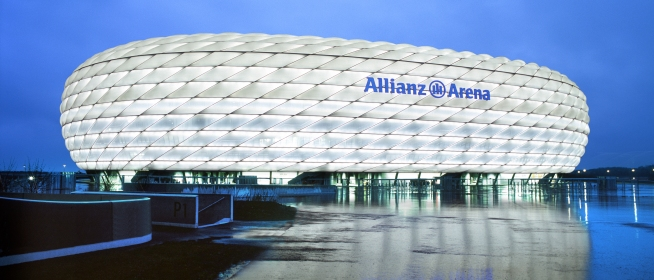
\includegraphics[width=0.31\textwidth]{./gfx/arena}
\caption{Den nye Allianz Arena, hjemmebanen til FC Bayern München}
\end{figure}

Du spør du deg kanskje hvorfor grensen er så lav, og dette er fordi det finnes en 20-timers-grense for studenter i Tyskland, så det skal unngås at studentene er mer på jobben enn de er på universitetet... Ferier og helger er utelatt fra denne 20-timers-grensen, så du regnet over hele året kan tjene 7235\euro{}. Det du tjener i Norge er ikke underlagt dette beløpet.
Har du to jobber må du ha et Lohnsteuerkarte til, og dette har da Steuerklasse 4. Her betaler du skatt, men får dette tilbakebetalt dersom du holder deg under den øvre grensen på 7235\euro{}.
Se disse sidene for mer informasjon: \\
\url{http://www.seezeit.com/opencms/export/download/Downloadgalerie_SozialesBeratung/Ich_und_meine_Rente.pdf} \\
\url{http://www.jobber.de/_1_myjobber/jobforum,arbeitsrecht.html}

\chapter{Fritid}


Fritiden er ikke vanskelig å fylle i en by som München. Museene og teatrene er allerede nevnt, men også konsertlokalene er mange og flotte, og det er mange verdenskjente artister som legger turen innom her når de er på turné. Alle statlige teater, operaer etc. har studentrabatt, og en kan oppleve mange flotte forestillinger for bare 5 euro. Olympiahalle og -stadion er litt større konsertarenaer for pop- og rockeartister. Det finnes også rikelig med klubblokaler som tilbyr litt mer intime konserter. Kinoer er det også nok av (også de som viser filmer på originalspråk), men det er jo de tyske kneipene som kaprer mest av fritida for mange. Det fins mange koselige kafeer og kneiper i hele byen. Vi norske bruker å være mest i bydelen Schwabing, som også karakteriseres som studentenes bydel. 


München arrangerte sommer-OL i 1972, og som et resultat av dette er tilbudene utrolig bra for studenter som liker å drive med sport og friluftsliv. I Olympiazentrum, den gamle olympiabyen, finnes det et stort sportskompleks (ZHS; Zentrale Hochschulsportanlage) som nå står til studentenes bruk. For 7,50 \euro{} pr semester har en fri tilgang til idrettshaller, fotballbaner, styrkerom, aerobic, basketball, badminton og alt annet sport en kan tenke seg.




Det finnes også 30 tennisbaner en kan bruke, men her må man betale litt i tillegg (2euro,- for en time pr. pers). ZHS arrangerer også skiturer, klatreturer og kurs i ALLE mulige sportarter. Se link nederst på neste side. Elles er det mange busselskap i byen som selger dagsturer (inkl. skipass) til Alpene for ca 30 euro. ANSA har dessuten noen semester arrangert fotballtrening/-moro hver fredag ettermiddag, der alle som har lyst stiller opp, gutter og jenter, trent som utrent, gode som ikke så gode. Ellers har jo München tre bundesligalag, de rike i FC Bayern München, det gamle arbeiderlaget TSV 1860 München, og de små frå Unterhaching. Så hver eneste lørdag kan man se dem i aksjon på Olympiastadion eller i nye Allianz Arena sammen med 69.900 andre tilskuere.
I en by som München kan en driva med alt, det er bare opp til en selv hvilket  miljø, hvilke organisasjoner og tilbud en oppsøker. 


\section{Oktoberfest og Starkbierfest}

Hvert år arrangeres Oktoberfest og Starkbierfest...




\section{Ski}
Fra München når man ganske enkelt noen av de flotteste skistedene i Alpene. Garmisch, Lengries, Wendelstein, Suedelfeld og (vår favoritt) Spitzingsee ligger alle ca en times kjøring unna.
Garmisch og Lengries kan nås med tog fra Hauptbahnhof.  Flere studenter benytter seg av dette tilbudet, som for en fast pris gir deg tog og dagskort til Garmisch. \url{http://www.s-bahn-muenchen.de/s_muenchen/view/aktuell/news/garmischer_ski_express.shtml} \\
Afterskien i de tyske alpene er ikke noe særlig. ``Studenten im Schnee'' ograniserer også turer for studenter til skiområder i Bayern, Zillertal, Tirol osv. Se \url{http://www.studentenimschnee.de/}


De østerriske alpene er heller ikke langt unna. Det første som møter deg er Zillertal, hvor du har Hochfügen, Mayrhofen og ikke minst Hintertux. Her er det bra skikjøring og god afterski. Spesielt i Mayrhofen. Du vil møte på en del hollendere og russere. Hintertux er en isbre, hvor en kan starte sesongen allerede i oktober. Afterski i hytta på parkeringsplassen er et must.





Hvis en beveger seg i rettning Salzburg, finner man steder som Kitzbühel, Ski Amade og snøhullet og kongeplassen Fieberbrunn hvor det er bra skikjøring, minimalt med turister og en hyggelig liten alpelandsby med greie priser.

Hvis en drar vestover, så finner man dal etter dal: Ötztal, Pitztal, Kaunertal osv., helt til man når Montafon, Ichgl, Sonnenkopof, St. Anton, Zürs og Lech i Voralberg. Her er det mye snø, og meget god skikjøring. Hvis en drar østover har man plasser som Bad Gastein, Obertauern og Kitzsteinhorn ved Zell am See.

Mulighetene for den som liker å stå på ski er mange. En av de beste internettsidene for å sjekke føreforhold og priser på overnatting er \url{http://www.bergfex.de/}. De har også en fra app for smartphones.

\begin{figure}[h]
\center
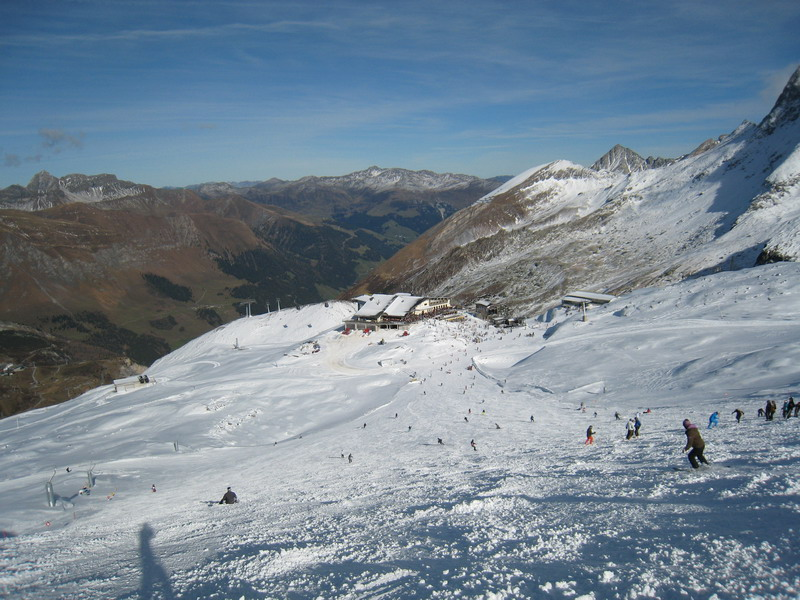
\includegraphics[width=0.31\textwidth]{./gfx/hintertux}
\caption{Tidlig sesong på Hintertux}
\end{figure}

\chapter{Annen nyttig informasjon}

\section{Oppholdstillatelse}
Ettersom Norge er en del av Schengen og EØS, trenger vi nordmenn kun å ta oss en tur til utlendingskontoret i rådhuset (Kreisverwaltungsreferat, U-Bahn Poccistraße) hvor vi får et dokument som sier "Jeg har lov til å være hær så lenge jeg vil". 

Her er internettsidene:\\
\url{http://www.muenchen.de/rathaus/Stadtverwaltung/Kreisverwaltungsreferat.html}

Ta med pass! Man blir spurt en rekke spørsmål, bla. bostedsadresse og religion.
Ta vare på dokumente(t)ne!
Det er her man også melder om flytting, innad i byen, men også hvis man flytter tilbake til Norge.

\begin{figure}[h]
\center

\includegraphics[width=0.31\textwidth]{./gfx/lech}
\caption{Alltid masse nysnø i Lech}
\end{figure}

\section{Forsikring}
Dette er noe mange ikke tenker på. Spesielt ansvarsforsikring er noe en bør har. Hvis en enda er forsikret hjemme i Norge gjennom foreldre eller foresatte så er saken grei. Men, hvis en skulle være så uheldig å forårsake en ulykke hvor en blir erstatningspliktig, sliter en uten ansvarsforsikring. ANSA tilbyr en meget god forsikringspakke med alt en trenger (ansvars-, innbo-, reiseforsikring etc.). En kan også skaffe seg ansvarsforsikring i Tyskland. Her heter det "Hauptpflichtversicherung". Flere studier vil kreve ansvarforsikring, ved f.eks. jobbe på lab. ANSA forsikring dekker ikke slikt, da vil man trenger å oppsøke et forsikringsselskap og forklare til hva, man trenger forsikringen. 

Forsikringsselskap: 
huk24.de
Allianz


Flere banker driver også med forsikring.


\section{Telefoni}

I Tyskland er det nesten som i Norge når det kommer til mobiltelefoner. Man kan kjøpe mobil med eller uten abonnement. Hvor man kan kjøpe mobil varierer, i store elektrokjeder som Saturn (tilsvarer Elkjøp og Bonus i Norge) der mobiler eller tilknyttet ulike typer abonnement, eller små telefonbutikker som er tilknyttet et abonnement (f.eks hvis Telenor hadde hatt sin egen butikk hvor det ble solgt mobiltelefoner med kun Telenorabonnement).
Hva som lønner seg mellom abonnement og kontantkort er helt avhengig av hvor mye du kommer til å ringe og hvor/hvem du ringer.
Man trenger som oftest en tysk bankkonto for å få et tysk mobilabonnement.

Vanligvis er man tilknyttet et abonnement 12-24 mnd. Dette er ganske lenge, og man må derfor tenke nøye gjennom hvilket abonnement man velger og hos hvilken leverandør.
En annen mulighet man har som er ganske spesielt i Tyskland er at man kan få ett mobilnr og ett eget "homezone"-nr. Denne "Homezonen" gjelder i 1 km omkrets fra der du bor og når du befinner deg der, kan du ringe med fasttelefonpriser fra "homezone"-nr ditt.. Spør forhandleren for ytterligere informasjon.
Det finnes veldig, veldig mange leverandører, noen leverandører er kun å finne på internett, disse pleier å være rimelig. En kort oversikt følger her:

De dyre: T-mobile (veldig lik Telenor)
 
De rimelige: Vodafone, O2 - studentenes favoritt,  callmobile.de. 

Disse tre har studenttariffer og kan bli ganske rimelig. O2 har til og med ubindende abonnemnt, som heller ikke er så dyr.
 
Fulliste finner dere her:\\
\url{http://www.verivox.de/handytarife/calculator.aspx}
 

Kontantkort anbefales de 2 første månedene av oppholdet ditt i Tyskland.
Er enkelt å få tak i, men kan også være den dyreste varianten. Hvis en ikke ringer så mye, er dette det greieste. Callmobile er forhåndsbetalt (pre-paid) som også tilbyr fri surfing for 10 euro i måneden.



\section{Internett}

M-net og Alice er de største operatørene på fast ineternett. De fleste universiteter tilbyr gratis trådløst nettverk, som man kan koble seg opp på fra sin egen laptop.


En oversikt over ulike firmaer som tilbyr internett finner du på denne siden:
\url{http://www.finanztip.de/preislotse/sonstiges/internet.php?phpurl=internetanbieter.php}

\begin{figure}[h]
\center
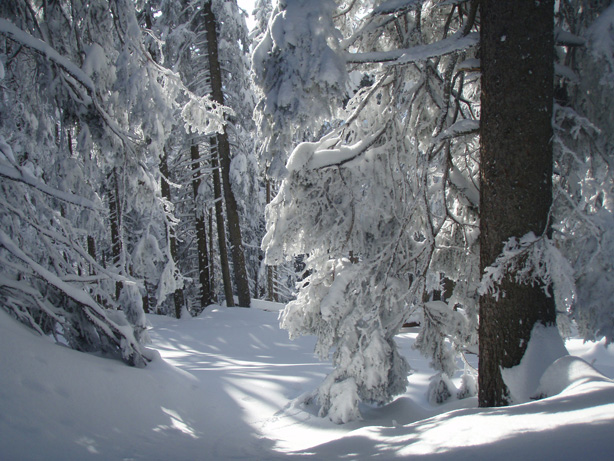
\includegraphics[width=0.31\textwidth]{./gfx/spitzing}
\caption{Klar for skogskjøring i Spitzingsee}
\end{figure}

\section{Bank}

Noe av det første man må skaffe seg når man flytter til Tyskland er en tysk bankkonto. For det første tar de færreste butikkene visa-kort, til og med ikea. For det andre krever f.eks. mobiloperatørene at man har en tysk konto. I Tyskland er det vanlig å bruke noe som heter EC-kort, men det er viktig å huske på at mange små butikker ikke tar kort i det hele tatt.
Når man velger bank er det viktig å tenke på at det koster å ta ut penger i andre banker/minibanker enn den man selv tilhører. Det vil si at det lønner seg å velge en bank med mange terminaler eller en i nærheten av der man bor. Deutsche Bank og Sparkasse er to banker som pleier å ha mange filialer i de fleste byene, og det er også mulig å få egne studentkontoer hos dem.
Man kan ikke bare droppe innom å opprette en konto, man må først bestille en time med banken for så å få en bankkonto. Husk pass.



\section{Kollektivtrafikk} \label{mvv}

München har et meget bra kollektivtilbud. By-tog (S-Bahn), undergrunnstog (U-Bahn), trikk (Tram) og buss.

Månedskort på MVV (Münchner Verkehrs- und Tarifverbund) koster fra 30 til 80 \euro{} uten studentrabatt, avhengig av hvor stort reisenett du trenger. Som immatrikulert student får man en rabarert månedsbillet.
Dette er relativt dyrt i forhold til andre tyske byer, selv med den lille studentrabatten en får på månedskort.

Se MVV for info:\\
\url{http://www.mvv-muenchen.de/de/tickets-preise/tickets/schule-ausbildung-und-studium/}


\section{Toll}

Har man tenkt å ta meg seg noe spesielt (bil, hund etc) fra Tyskland til Norge eller omvendt, kan det være lurt å ta seg en titt på \href{http://www.toll.no}{www.toll.no} eller  \href{http://www.zoll.de}{www.zoll.de} først.

En kan også sjekke mulighetene for utføre varer momsfritt. Ettersom vi er studenter og som oftest kun har registrert en postadresse i utlandet, faller vi litt mellom to stoler. Vi kan lovlig få tilbake norsk moms på varer kjøpt i norge ved utførsel (som turister). Se \url{http://www.toll.no/templates_TAD/Topic.aspx?id=256215&epslanguage=no}. \\
Det greieste er alternativ 1: Print ut skjema, og fyll inn detaljene. Skjema med kvittering stemples hos tollvesenets skranke når en drar tilbake til Tyskland på flyplassen. Husk å gjøre dette før du sjekker inn bagasjen, hvis varen du skal utføre ligger der.\\
Orginal skjema med kvittering sender du så til butikken du kjøpte varen, påført ditt kontonummer, og du får tilbakeført merverdiavgiften.


En kan også gjøre dette når eg har kjøpt en vare i Tyskland, og reiser hjem til Norgei. Dette er muligens ikke helt etter boka, men går så lenge man sier at man kun har vært på besøk i Tyskland (ikke registrert adresse). Skjema er meget likt det norske: \url{http://www.zoll.de/SharedDocs/Downloads/DE/FormulareMerkblaetter/Privatpersonen/steuer_2004.pdf?__blob=publicationFile}. \\
På flyplassen sjekker man ikke inn bagasjen, men nevner at man skall innom tollvesenet. Tollvesenet må da se varen og stemple dokumentet samt kvittering før de sender inn bagasjen din fra deres eget transportbånd. \\
All informasjon finner du her: \url{http://www.zoll.de/DE/Privatpersonen/Reisen/Reisen-nach-Deutschland/Zoll-und-Steuern/Tax-free-einkaufen/tax-free-einkaufen_node.html}



\framebreak
\framebreak
\vspace{4cm}

\large
Vi håper denne guiden gir deg noe av den informasjonen du søker, enten du faktisk skal til München eller lurer på å komme hit. Det er ikke gjort på en kveld å sette seg inn i alt en må tenke på før en skal flytte. Ta en ting om gangen og begynn forberedelsene tidlig.

Hvis det er noe mer du lurer på, kan du ta kontakt med en av våre kontaktpersoner:
\begin{itemize}
\item{Ludwig-Maximilians-Universität München}\\
Vemund Vikjord \\
\href{mailto:v.vikjord@live.no}{v.vikjord@live.no} 

\item{Technische Universität München}\\
Peter Netland \\
\href{mailto:mr.netland@hotmail.com}{mr.netland@hotmail.com} 
\end{itemize}

\vspace{1cm}

Vi håper å se deg i München!


\vspace{2cm}

Beste hilsen,\\
Stavanger \hfill Henrik Nyhus \\
München \hfill Peter Netland \\
Juli 2013








\framebreak
\chapter{Linker}


\url{http://www.ansa.no/ANSAland/Tyskland/Studenter/Studieinteresserte/}\\
En del praktisk opplysninger om det å flytte til Tyskland, se emner i venstre marg.

\url{http://www.ansa.no/upload/Landsbrosjyre_Tyskland-2012.pdf} \\
ANSAs brosjyre om Tyskland; mye nyttig informasjon om søknadsprosessen.

\url{http://www.zhs-muenchen.de} \\
Sportprogrammet for alle studenter i byen.

\url{http://www.facebook.com/group.php?gid=2244635897} \\
Facebook-gruppen vår.

\url{http://www.fromnorth.de} \\
Hovedsakelig Finner og Svensker.

\url{http://www.norwegerinbayern.de} \\
Norske familier og ikke-studenter.

\url{http://www.toytowngermany.com} \\
Forum for internasjonale i München, bra side.

\url{http://www.norwegisches-konsulat-muenchen.de} \\
Det Kgl. Norske Konsulatet.

\url{http://www.in-muenchen.de} \\
Konserter, fester osv.

\url{http://www.muenchen.de} \\
Byens offisielle internettside.

\url{http://www.heinzelnisse.info} \\
Bra gratis ordbok.

\url{http://de.wikipedia.org/wiki/München}

\url{http://www.daad.de} \\
Iinformasjon om tysk utveksling





 
 	

\clearpage
\tableofcontents
\label{lastpage}

\end{document}
